\documentclass[10pt, a4paper, egregdoesnotlikesansseriftitles]{scrartcl}


% initialize packages and macros
% general math/drawing stuff
\usepackage{geometry}
\usepackage{mathtools}
\usepackage{hyperref}
\usepackage[]{graphics}
%\usepackage{tikz}      -- see tikz section
%\usepackage{pgfplots}
\usepackage{amsmath, amssymb}

% Packages for algorithms/code -- copied, possibly unnecessary
\usepackage{listings}
\usepackage{verbatim}
\usepackage{algorithmicx}
\usepackage[noend]{algpseudocode}
\usepackage{algorithm}
\algdef{SE}[DOWHILE]{Do}{doWhile}{\algorithmicdo}[1]{\algorithmicwhile\ #1}%

% nicer author management
%\usepackage{authblk}

% colorsssss
\usepackage[dvipsnames]{xcolor}
% define your colors at the end

% drawing tools
\usepackage{tikz}
\usepackage{pgfplots}
\pgfplotsset{compat=1.16}
% add all required graph elements here
\usetikzlibrary{arrows.meta, automata, backgrounds, shapes, decorations}
\usetikzlibrary{positioning,fit,calc}  
\tikzset{
        block/.style={draw, thick, text width=3cm, minimum height=1.5cm, align=center},   
        line/.style={-latex}
    }

% useful common symbols idk copied em
\newcommand{\booleans}{\mathbb{B}}
\newcommand{\naturals}{\mathbb{N}}
\newcommand{\integers}{\mathbb{Z}}
\newcommand{\ordinals}{\mathbb{O}}
\newcommand{\numarals}{\mathbb{I}}
\newcommand{\reals}{\mathbb{R}}

\newcommand{\maps}{\rightarrow}
\newcommand{\pmaps}{\hookrightarrow}

\newcommand{\union}{{\cup} }
\newcommand{\Union}{{\bigcup} }
\newcommand{\powerset}[1]{2^{#1}}
\newcommand{\intersection}{{\cap} }
\newcommand{\intersect}{\intersection}
\newcommand{\Intersection}{{\bigcap} }
\newcommand{\compose}{{\circ} }


\newcommand{\ltrue}{\mathbf{tt}}
\newcommand{\lfalse}{\mathbf{ff}}
\newcommand{\limplies}{\Rightarrow}
\newcommand{\lxor}{\oplus}
\newcommand{\Land}{\bigwedge}
\newcommand{\Lor}{\bigvee}
\newcommand{\Lxor}{\bigoplus}
\newcommand{\lequiv}{\Leftrightarrow}
\newcommand{\landplus}{\mathrel{:\hspace{-3pt}\land\hspace{-3pt}=}}
\newcommand{\lorplus}{\mathrel{:\hspace{-3pt}\lor\hspace{-3pt}=}}
\newcommand{\bigO}{\mathcal{O}}


% author notes
\newcommand{\pushkar}[1]{{\color{Aquamarine} Pushkar: #1}}
\newcommand{\sankalp}[1]{{\color{RubineRed} Sankalp: #1}}


% colorssssss
\definecolor{test}{HTML}{FF0000}

% general macros go here
\newcommand{\petris}{\texttt{petris}}


% allow a figure to be broken across columns and pages
% its absence is a source of sheer annoyance - sg
\allowdisplaybreaks{}
\geometry{a4paper, textwidth=6.3in}

\title{$\petris$}
\subtitle{A Tetris Clone}

% Authors, ordered by roll num
\author{
    Pushkar Mohile \\
    $\texttt{180260027}$
    \and
    Sankalp Gambhir \\
    $\texttt{180260032}$
    }

\date{June 2020}

\begin{document}

\maketitle

\begin{abstract}
    \centering
    $\textbf{Abstract --}$
    $\petris$ is a bad attempt at a portmanteau of 
    EP and Tetris. It recreates the classic game of Tetris on a hardware simulation. We have developed a game module and a VGA simulator using the SDL library. 
\end{abstract}

% section names copied from the format from now, subject to change
  
\section{Project Details}
% description of block structure 

% block diagram
\begin{figure}
    \centering
    
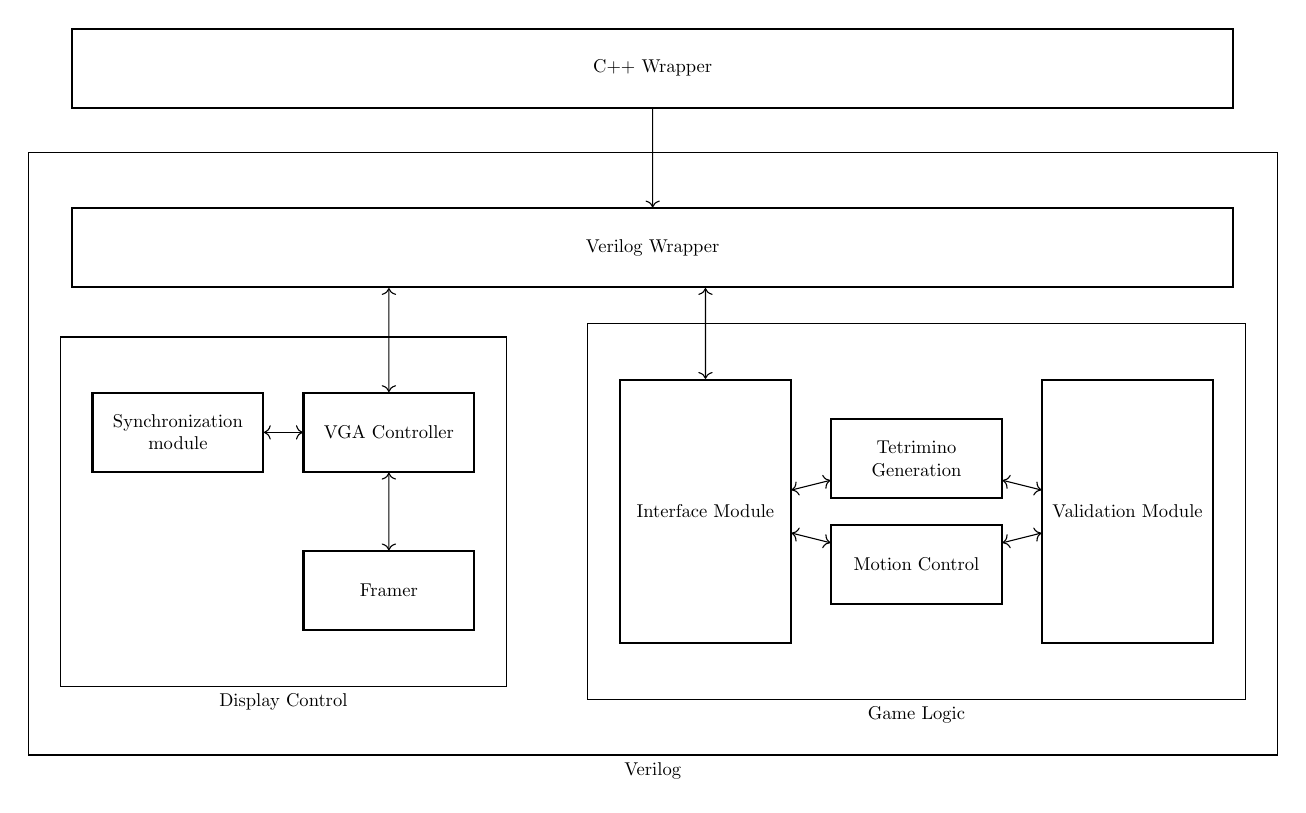
\begin{tikzpicture}[scale=0.67, every node/.style={transform shape}]
    % macro block diagram for simulation

    \node[block, minimum width=22cm ] (cpp) at ( 2,  0.9) {C++ Wrapper};
    
    % blocks part of the display super-module
    \node[block, minimum width=22cm ] (main) at ( 2, -2.5) {Verilog Wrapper};
    \node[block] (sync) at (-7, -6) {Synchronization module};
    \node[block] (vga) at (-3, -6) {VGA Controller};
    \node[block] (fr) at (-3, -9) {Framer};
    
    % blocks part of the logic super-module
    \node[block, minimum height=5cm] (int) at ( 3, -7.5) {Interface Module};
    \node[block] (tetgen) at ( 7, -6.5) {Tetrimino Generation};
    \node[block] (motcon) at ( 7, -8.5) {Motion Control};
    \node[block, minimum height=5cm] (val) at ( 11, -7.5) {Validation Module};

    \node[draw,inner xsep=4mm,inner ysep=7mm,fit=(vga)(fr)(sync), label={-90:Display Control}] (d) {};
    \node[draw,inner xsep=4mm,inner ysep=7mm,fit=(int)(tetgen)(motcon)(val), label={-90:Game Logic}] (l) {};
    
    \node[draw,inner xsep=4mm,inner ysep=7mm,fit=(main)(d)(l), label={-90:Verilog}] (v) {};

    % super-module connections
    \draw[->] (cpp)-- (main);
    \draw[<->] (vga)-- (vga|- main.south);
    \draw[<->] (int)-- (int|- main.south);

    % display connections
    \draw[<->] (vga.west)-- (sync.east|- vga.west);
    \draw[<->] (fr)-- (vga);

    % logic connections
    \draw[<->] (tetgen)-- (int);
    \draw[<->] (motcon)-- (int);
    \draw[<->] (tetgen)-- (val);
    \draw[<->] (motcon)-- (val);

\end{tikzpicture}

    %\captionsetup{justification=centering}
    \caption{Block diagram $\sankalp{Better caption?}$}
\label{fig:blockdiag}
\end{figure}

% verilog
\subsection{Verilog Modules}

% wrapper
\subsubsection{Wrapper}


% logic supermodule
\subsubsection{Logical Modules}

\paragraph{Interface Module}
\paragraph{Tetrimino Generation Module}
\paragraph{Motion Control Module}
\paragraph{Validation Module}

% display supermodule
\subsubsection{Display Modules}

\paragraph{VGA Control Module}
\paragraph{Framer Module}
\paragraph{Synchronisation Module}


% c++
\subsection{C++ Wrapper}

\section{Main Components}
\subsection{I/O Modules}

\subsection{Hardware Description}
\subsection{Structural Description }
\subsection{Behaivoural Decription}
The physical components to develop this project would be 
\begin{itemize}
    \item An FPGA
    \item A VGA Display
    \item A DAC to feed the output of the FPGA to the VGA
    \item Buttons to control the inputs 
    \item A laptop with the Intel Quartus software and the required connecters. 
\end{itemize}}
We would expect this to be somewhat easier as we would only have to focus on the game logic and the I/O should
 be substantially simpler. 

\section{Results}

The game works as intended with the operations being correctly evaluated
 and the gameboard updating correctly to reflect all the changes. The score updates correctly on deletion of full rows, with greater weights 
being given to deleting more rows simultaneously. The game correctly ends on any coloumn being filled. \\
A quick gameplay run showing this can be seen in the video linked at:

\begin{align}
    \centering
    \textnormal{\url{https://shorturl.at/etvQ9}} \nonumber
\end{align}

\begin{figure}[ht]
    \centering
    \begin{subfigure}[b]{0.4\textwidth}
        \centering
        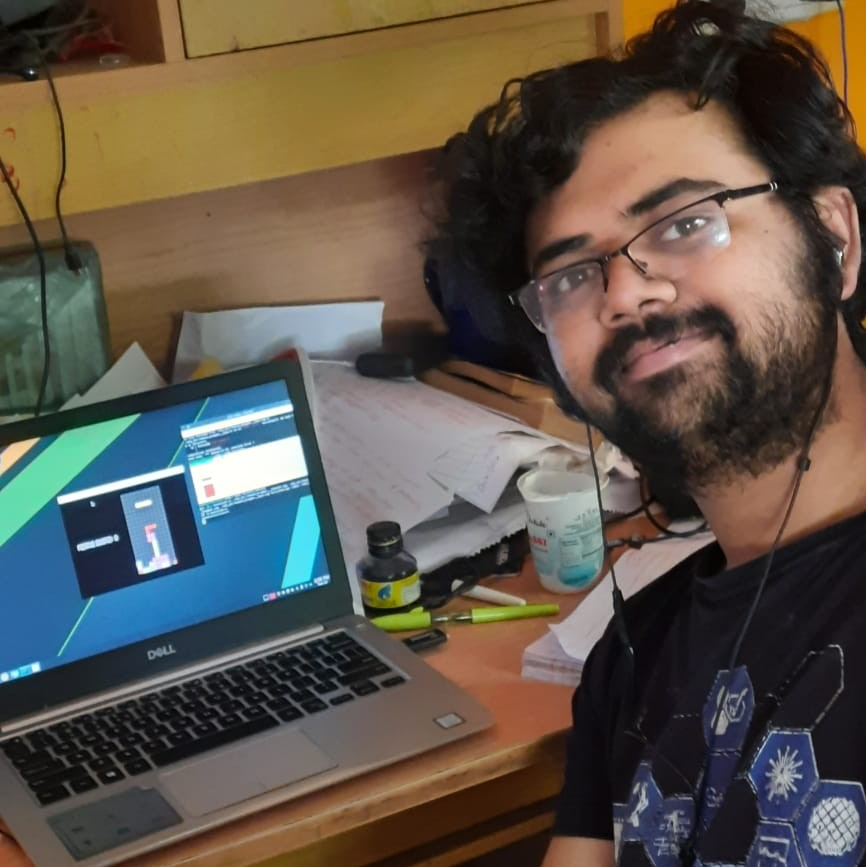
\includegraphics[width=\textwidth]{fig/demo-pushk.jpeg}
    \end{subfigure}
%
    \begin{subfigure}[b]{0.4\textwidth}
        \centering
        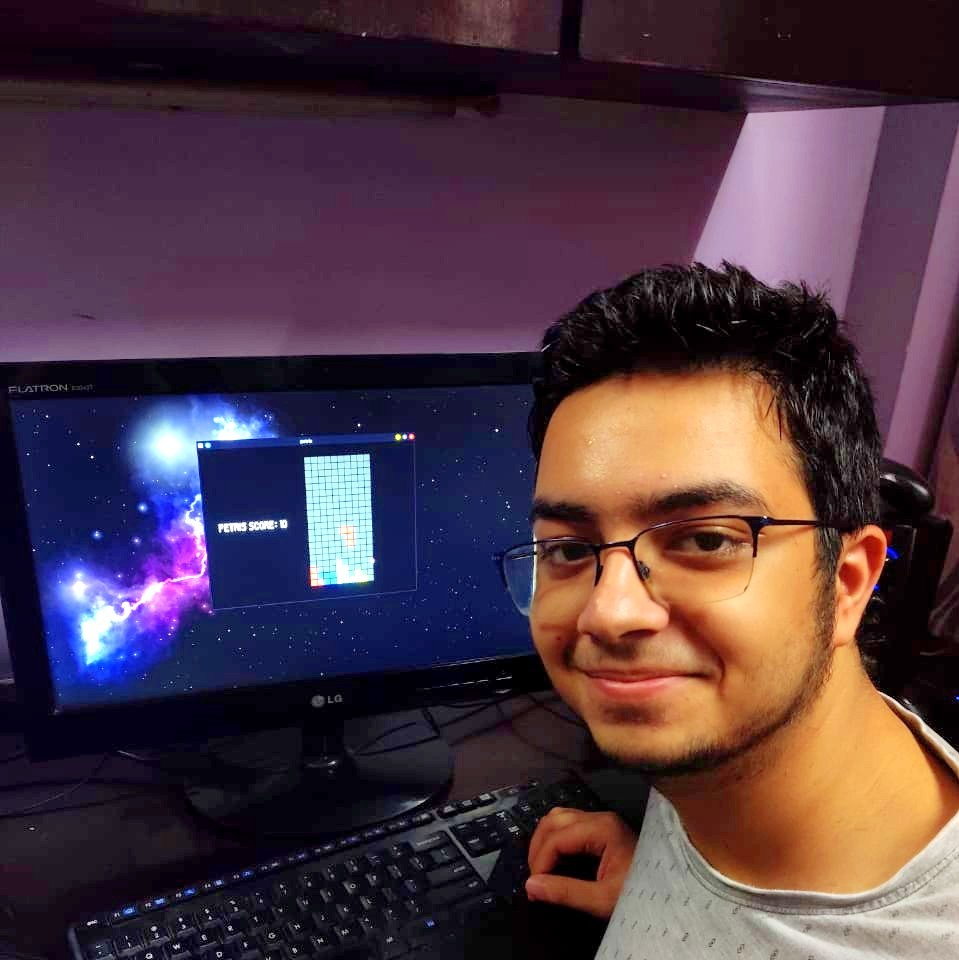
\includegraphics[width=\textwidth]{fig/demo-sank.jpeg}
    \end{subfigure}
    \caption{\emph{Look Ma! No FPGA!}}
\label{fig:demo}
\end{figure}


There are several optimizaions and additional features that can be implemented. Implementations to the User Interface could include
\begin{itemize}
    \item A game reset button that allows you to play multiple games on one execution
    \item A high score display that keeps track of your best performances
\end{itemize}
Potential optimizations to the game would include
\begin{itemize}
    \item Improving the framerate of the VGA simulator
    \item Introducing more parallel updating for the game logic, which it is currently not due to synchronization and framerate issues. This currently doesn't matter 
     due to the low framerate being the rate determining step but this should definitely be done if using a real FPGA 
\end{itemize}

The project can be found at our GitHub repository: \url{https://github.com/sankalpgambhir/petris}.



\end{document}